% needs IEEEtran.cls
%
\documentclass[10pt,journal,compsoc]{IEEEtran}
%\documentclass[conference,compsoc]{IEEEtran}

\usepackage{graphicx}% Include figure files
%\usepackage{bm}% bold math
%\usepackage{gensymb}


%%%%%%%%%%%%%%%%%%%%%%%%%%%%%%%%%%%%%%%%%%%%%%%%%%%%%%%%%%%%%%%%%%%%%%%%%%%%%%%%
%%%%  Body of document follows...
%%%%%%%%%%%%%%%%%%%%%%%%%%%%%%%%%%%%%%%%%%%%%%%%%%%%%%%%%%%%%%%%%%%%%%%%%%%%%%%%
\begin{document}

\title{Quantum Time Signals in Living Beings}

\author{Brad Eckert}
%\email{hwfwguy@gmail.com}
%\affiliation{Iolera Holdings LLC}

\date{\today}% It is always \today, today,
             %  but any date may be explicitly specified


\IEEEtitleabstractindextext{%
\begin{abstract}
Consciousness is considered a physical process occuring inside and outside of time simultaneously,
per spiritual traditions and modern QM theory, using two-dimensional time.
Quantum time hypothetically emerges from non-local consciousness as it interacts with both worlds.
The relationship between the time dimensions provides a mechanism for apparent
noise arising from both our biological signaling and connection to ``divinity''.
We present an algorithm for the demodulation of white and pink noise,
which could have ``hidden'' information content that instruments the
mind-body landscape.
If found, the demodulated signals would facilitate a new class of consciousness applications.
The detection and analysis of these signals, or instrumenting the soul,
would have far-reaching implications for social structures, governance, and public health.
\end{abstract}


% Note that keywords are not normally used for peerreview papers.
\begin{IEEEkeywords}
Tao, flicker noise, emergent time, consciousness, QTDSP.
\end{IEEEkeywords}}

\maketitle

%\tableofcontents

\section{\label{sec:level1}Two-Dimensional Time}

According to most spiritual traditions, the consciousness of humans, animals,
and all living things is a combination of the finite and the infinite,
both inside and outside of material reality.
This view is allowed by theoretical physics.

The Wheeler-DeWitt equation \cite{DeWitt} attempts to combine mathematically
the ideas of quantum mechanics and general relativity.
One of its implications is the ``problem of time'',
which is a conceptual conflict between general relativity and quantum mechanics.
Quantum mechanics regards the flow of time as universal and absolute, whereas
general relativity regards the flow of time as malleable and relative.

According to Wheeler-DeWitt, an observer outside of the universe
doesn't experience time. Page and Wooters \cite{Page} addressed this paradox
(time \textit{seems} real enough) by treating time as an emergent phenomenon
resulting from quantum entanglement.
Experiments \cite{Moreva} on entangled particles have bolstered the theory.

There are other takes on timeless universe models. 
Aharonov's two state formalism of quantum mechanics has also been used
\cite{Lobo} to propose emergence of time from a timeless unus mundus
quantum-like space.
Jianfeng Li provides a good overview \cite{Jianfeng} of quantum mechanical
timeless consciousness.

There are two distinct types of time: emergent time, which emanates from the
structure of space-time and its metrics, and a causal time, indicating the flow
from the past to the future \cite{Brunet}. The time domains boil down to the
two models of Physics, QM and GR. 
In the interest of a nomenclature for the masses, we call one dimension of time
the quantum time domain and the other the relative time domain. 
So, quantum time and relative time. Relative time is the one with the arrow.

The hard problem of consciousness \cite{Chalmers} is that of explaining the
relationship between physical phenomena, such as brain processes,
and experience.
Experiments in non-locality \cite{Achterberg} find that the mind extends beyond
the skull. Where is the mind, inside space-time or outside?
The evidence suggests it is both.

Our everyday experience is that ``clock time'' is the static reference frame,
although it could just as well be that quantum time is the existential norm
and the ``clock time'' universe is the special case.
We take the view of quantum time observed from within the universe, with
the observation being an act of quantum entanglement caused by consciousness.

\subsection{Quantum Time and Consciousness}

There are many examples of biological systems exploiting quantum effects.
Nature would have evolved to exploit the properties of quantum time.
Let's allow the ``woo'' to ride for the moment, seeing as how the actual
physics can be filled in as the science unfolds. Isn't it always?

The physical vacuum, or classic Tao, a substrate for quantum interactions,
is a natural mechanism for biological systems to have evolved to utilize.
Consciousness is the interaction between the physical vacuum and biology which
facilitates communication and data storage at any physical scale,
from DNA to organism.

This provides an important signaling mechanism for consciousness in beings such
as paramecia that are too small for consciousness to arise from network effects.

One way to relate the two time dimensions is with a scale-invariant geometry
that exploits the simplicity of self-similarity.
As Mandelbrot \cite{Mandelbrot} pointed out, relatively simple fractal
mathematics underlie many complex natural phenomena.
As it turns out, this exponential relationship between $\tau$ and $t$
is a key enabler of signal transformations.

For it to be scale invariant,
we use an exponential growth model for quantum time.

\begin{equation} \label{eq:pink}
\tau \propto e^{\epsilon t}
\end{equation}

The mechanics of signal generation can be considered in the context of
quantum time.
This arrangement lends itself to information flow, utilized by nature,
between the time and timeless domains.

Resonance is treated as a physical phenomenon occurring in quantum time $\tau$.
A resonant frequency in $\tau$ is equivalent to an exponential chirp in $t$.
This dynamic emergence of time should produce small but detectable artifacts.
The stream of consciousness emerges from a probabilistic field on an
exponential time scale rather than time abruptly appearing from nothing.

Biological systems evolve to minimize the expenditure of energy. Resonances
(field analogs of electrical and mechanical ringing) require a small energy
input to keep them going, assuming a reasonably high Q. It stands to reason
that biological systems would use field resonances in the physical vacuum
(the exact nature of the field needs not be understood)
to transmit consciousness information efficiently.

In other words, there is a theoretical basis for the notion that
``It's all vibrations''.
The vibrations occur in quantum time, so that summing the signal artifacts
from a large number of them results in a noise spectrum.

The signals that encode this information can be demodulated from flicker noise.
The information of consciousness can then be a new media,
to augment other forms of electronic media,
enabling new ways of being that improve individuals and society.

\section{Exponential Flicker Noise}

Flicker noise (or 1/f noise), has a power spectrum proportional to
$1/f^{\alpha}$, where $\alpha$ is between 0.7 and 1.4.
It's a type of noise prevalent in many natural systems.
Flicker noise \cite{Milotti} is seen in music, seismic data, EEG and ECG data,
and electronic devices.
Some of the more popular explanations for the 1/f spectrum are:
\begin{itemize}
	\item A superposition of relaxation processes.
	\item Carrier mobility fluctuations through Coulomb scattering.
\end{itemize}
There are a good number of hypotheses for 1/f noise, to which we add one more:
\begin{itemize}
	\item The superposition of exponential chirps.
\end{itemize}
A single exponential chirp has a power spectrum,
with ``warp factor'' $\omega$, of:
\begin{equation}
Power \propto |\omega| e^{-|\omega|f}
\end{equation}
A distribution of chirps of various $\omega$ values exponentially distributed,
where $log(|\omega|)$ is uniformly distributed, combines to form a 1/f spectrum.
So, there is a plausible basis for 1/f noise being composed of exponential
chirps.

The 1/f spectrum suggests that a multiplicity of quantum time rates
($\epsilon$ in Eq.~\ref{eq:pink}) exist.
Nature evolves to fill the spectrum of quantum time, to utilize available
bandwidth. One could call this spectrum ``The sound of the Tao''.
Music in the $\tau$ domain would sound like pink noise in the $t$ domain.

\subsection{Exponential White Noise}

White noise has a flat power spectrum.
In a white noise model of quantum time, chirps start at 0 and asymptotically
approach a final frequency as quantum time merges into relative time.

\begin{equation} \label{eq:white}
\frac{1}{\tau} \propto (1-e^{-\epsilon t})
\end{equation}

In other words, the consciousness signal emerges from a domain of infinite time.
The amplitude drops off with time at the same rate frequency increases,
resulting in a flat spectrum from DC to $f_0$.

\begin{equation}
f = f_0 \cdot (1-e^{-\epsilon t})
\end{equation}
\begin{equation}
a = a_0 \cdot e^{-\epsilon t}
\end{equation}

$f_0$ would be millimeter wave (such as 60 GHz oxygen resonances) and higher.
Terahertz (mostly in the 600 THz range) oscillations in tubulin \cite{Craddock}
correlate with anesthetic potency, which infers that
tubulin oscillations could be carriers of consciousness information.

The chirp should mix with carrier $f_0$ to produce a downward chirp
compatible with the flicker noise model.
That may be a more practical way to detect it due to the shortness of the
time the chirp itself spends in a bandwidth that lends itself to detection.

This paper presents the flicker noise model, which is more practical due to
its scale invariance.

\subsection{Information in the Noise}

Since exponential chirps are bounded in time, a single chirp has a finite
existence. It corresponds to a discrete impulse in the relative time domain,
or one symbol of information.
The idea of consciousness as time quanta may be useful here.
The act of being is a stream of consciousness that has corresponding streams
of pulse-coded information, a kind of informational counterpart to DNA.
The impulse stream may be decoded for its information content.
The existence of an impulse stream itself is valuable,
regardless of our initial ability to decode it, because useful information
can be mined from its distribution of $\omega$ values.

Consciousness quanta have a foundation in Penrose and Hameroff's
``Orch OR Theory'' \cite{Hameroff}.
In objective reduction, the divergence of quantum superposition in the
underlying structure of the universe builds to the point of collapse,
or objective reduction of the quantum state.
Each collapse is a moment of conscious experience.
In ``Orch OR'', EEG is a macro view of these moments.
EEG has both a flicker noise spectrum and frequency peaks that correspond
to ``Orch OR'' collapse.
There is already much scientific data (such as EEG and ECG studies) in the
public domain, ready to analyze.
The experimental costs are low: mostly computer hardware.

Overlapping chirps can be re-sampled and self-correlated to construct a relative
time domain signal for one or a multiplicity of $\omega$ values.
A sweep of $\omega$ can be used to construct a ``warp spectrum'' (for example,
on a computer display), useful for finding quantum-time signals.
This would be analogous to waterfall-style spectral analysis, with frequency
replaced by warp factor.

To establish a notation and unit of measurement for the exponent of the chirp
frequency, let the ``warp factor'' $\omega$ be in units of $e$, the
mathematical constant derived by Leonhard Euler in the 1720s, per unit time.
The pronunciation may be ``e's per second'' for e/s, for example.
We propose ``len'' for the unit name of e/s, after Leonhard.
Some scale factors to other units: 0.69 lens is one octave per second,
2.3 lens is one order per second, and 0.48 lens is one golden mean
$(\Phi=1.618:1)$ per second.
Note that a len is very close to twice the Golden Ratio,
so one must be careful when making assumptions about Golden Ratio relationships
in nature.

%%%%%%%%%%%%%%%%%%%%%%%%%%%%%%%%%%%%%%%%%%%%%%%%%%%%%%%%%%%%%%%%%%%%%%%%%%%%%%%%
\subsection{Spiral Conceptual Model}

\begin{figure}[h]
	\centering
	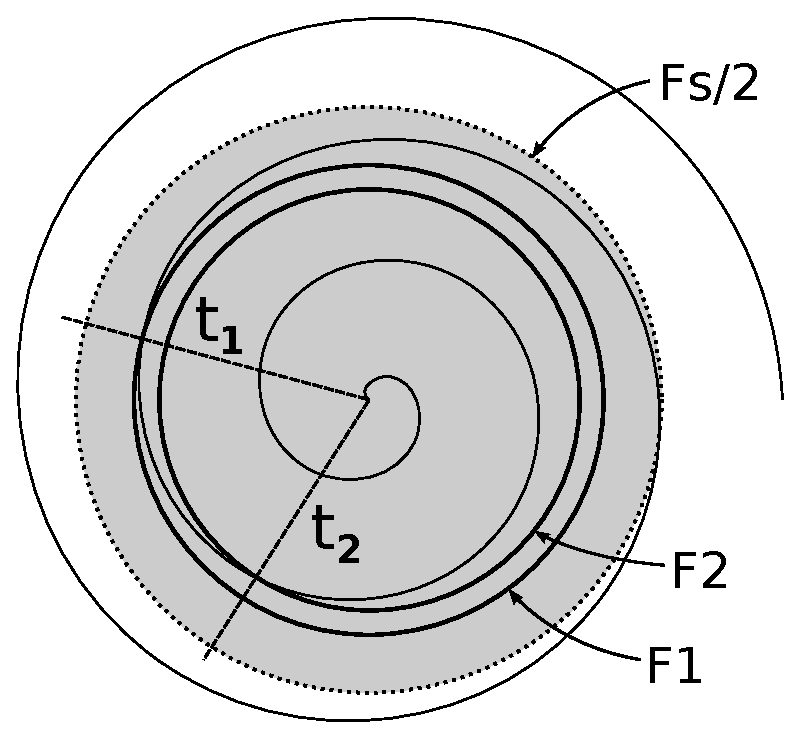
\includegraphics[width=0.7\linewidth]{../source/spiral_e}
	\caption[Quantum to Relative Time Relation]{Log polar plot of exponential chirp}
	\label{fig:spiral}
\end{figure}

Resonant signals in the quantum time domain can be re-mapped to relative time
and demodulated by correlating a time series of fast exponential chirp
transforms, allowing analysis and data mining using modern data
processing technologies such as AI-based pattern recognition.

The correlation effect can be visualized as a spinning logarithmic spiral
illuminated by a strobe light. When the strobe frequency matches the rate
constant of the spiral(s), it appears to be standing still.
Otherwise, it's a blur.

The relationship between quantum time and relative time can be thought of as a
2D plot in log-polar format.
Log-polar format renders a logarithmic spiral as a linear (Archimedean) spiral.
The spiral's radius is $\rho = k\theta$, where $k$ is a rate constant.
$\rho$ can represent either time or frequency by flipping the sign of $k$.
For purposes of signal processing, let $\rho$ represent log frequency and
$\theta$ relative time.

Log-polar mapping has proven useful in machine vision \cite{Bonmassar}
because it approximates the primate visual map \cite{Schwartz}.
Humans are visual thinkers, so their waking consciousness should map onto the
log-polar structure of quantum time signaling.

Fig.~\ref{fig:spiral} plots an exponential chirp in log-polar format.
A line can be drawn outward from the center of the spiral, crossing it at
multiple points.
The line rotates clockwise (in the case of downward chirp) at a step size
(from $t_1$ to $t_2$) corresponding to the oversampling rate.
For example, if the oversampling rate is 36 (each input value is used 36 times),
the step size is $10^{\circ}$.
Each angular sweep of the unit circle
(beginning and ending at line $t_1$ or $t_2$)
represents the input to a version of the Mellin transform called the
``Exponential Chirp Transform'' (ECT) \cite{Bonmassar}, which is
basically a FFT with time-warped input.

The transform's frequency domain output is along line $t_1$ or $t_2$ from
approximately $\rho$ = 0 to Fs/2, where Fs/2 (the Nyquist frequency)
is shown by the dashed circle.
The radius of the circle represents the approximate bandwidth of the system.
Not all of the circle is used: Anti-aliasing cuts off before Fs/2, while signal
near the center is too spread out to be useful.

The ECT time-warps the chirp signal, which represents a single ``quantum tone".
In the $360^{\circ}$ sweep at line $t_1$,
the chirp is time-warped to a tone F1 in relative time.
A time $t_2-t_1$ later, at line $t_2$,
it's time-warped to a tone of frequency F2.
All time warping is exponential.
Note that ``exponential time warping'' is different from dynamic time warping,
a popular means of pattern-matching mostly linear signals.

A convenient side effect of time warping is to transform interference
(periodic signals) into wideband noise.
The usual frequency peaks of EEG and HRV are thus discarded.

Quantum time, being logarithmic, has the property of frequency going as
$-\tau$ rather than $1/t$.
To change between time and frequency, just flip the sign of the exponent.
Tones are mirror images of time.
Signal processing is more convenient in terms of frequency,
so that is the focus of this paper.

%%%%%%%%%%%%%%%%%%%%%%%%%%%%%%%%%%%%%%%%%%%%%%%%%%%%%%%%%%%%%%%%%%%%%%%%%%%%%%%%
\subsection{\label{sec:level1}Quantum Time DSP}

The basic data flow of signal conversion from one time domain to another
$(\tau \leftrightarrow t)$ is shown in Fig.~\ref{fig:sled}.
The conversion algorithm slides along the input and output data streams,
forward in time.
Data is processed in overlapping chunks.
In other words, after a block of processing,
the sliding part of Fig.~\ref{fig:sled} shifts slightly to the right.
In proportion to the amount of shift,
new input stream is exposed and new output stream is completed.
The I/O streams are low-bandwidth compared to the compute-intensive
processing block.

\begin{figure}
	\centering
	\includegraphics[width=0.95\linewidth]{../source/sled_e}
	\caption[Quantum to Relative Time Translation Flow]{Inter-domain data flow}
	\label{fig:sled}
\end{figure}

There are two use cases: demodulation and modulation.
For demodulation $(\tau \rightarrow t)$, the input stream is in the quantum
time domain and the output stream is in the relative time domain.
The downsampler decimates the input by 1:m, where decimation factor m is
exponentially swept upward from or downward to 1.0.
The ``warp factor'' is the growth rate in m.
The input stream consists of real numbers.
The FFT performs a real-to-complex FFT to produce a warped spectrum which is
treated as a time-domain envelope of magnitude and phase information.
To un-warp the spectrum, the upsampler interpolates it by 1:m where decimation
factor m is exponentially swept upward to or downward from 1.0.
The output stream consists of vectors that are many accumulations of overlapped
upsampler results.

For modulation $(t \rightarrow \tau)$, the input stream is in the relative time
domain and the output stream is in the quantum time domain. The downsampler
decimates the input by 1:m, where decimation factor m is exponentially swept
upward from or downward to 1.0 and the resulting spectrum ranges from about
N/5 to N/2.
The ``warp factor'' is the growth rate in m.
The input stream consists of complex numbers.
The IFFT performs a complex-to-real IFFT to produce a warped time domain
envelope. To un-warp the it, the upsampler interpolates it by 1:m
where decimation factor m is exponentially swept upward to or downward from 1.0.
The output stream consists of many accumulations of overlapped upsampler results.

The usual use case is demodulation.
Modulation could be for testing, reconstruction or extrapolation of a signal,
or modulation of an energy source for yet unknown applications.


\section{QT Demodulation}

\begin{figure}
	\centering
	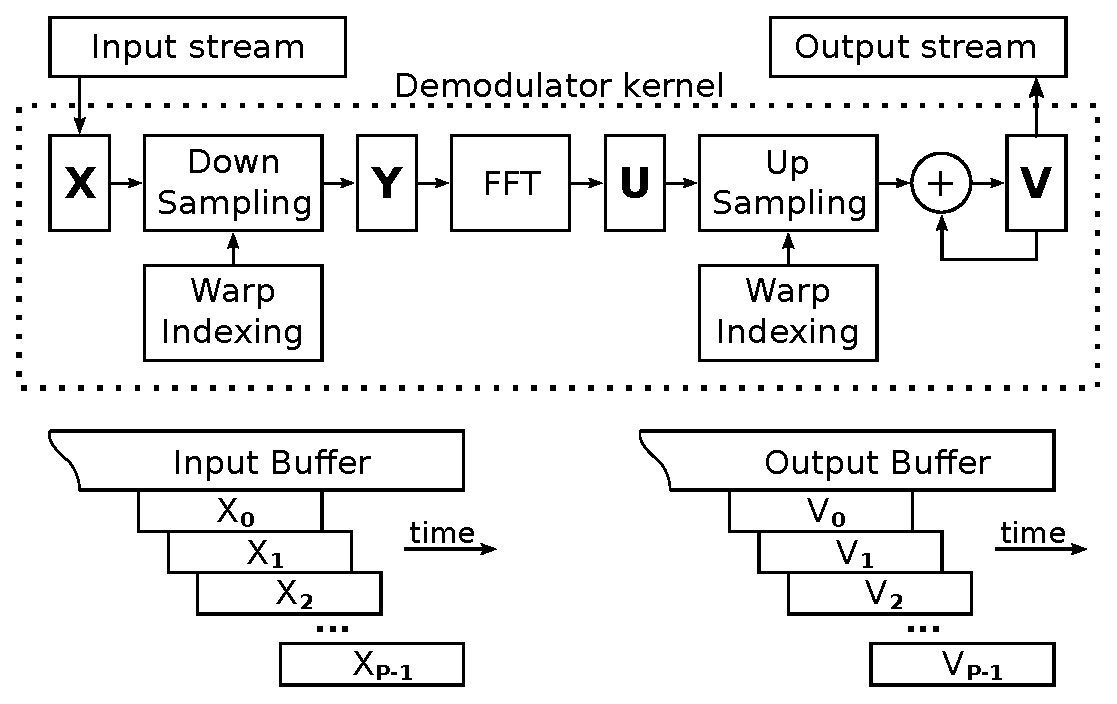
\includegraphics[width=0.95\linewidth]{../source/demod_e}
	\caption[Quantum to Relative Time Demodulation]{Demodulation data flow}
	\label{fig:demod}
\end{figure}

\begin{table}
	\label{tab:memory}
	\caption{Memory regions X, Y, U, and V in Fig.~\ref{fig:demod}
	are working buffers. For a 1k RFFT computed in place, the total is 11kB:}
	\centering
	\begin{tabular}{lccr}
		\hline\hline
		Buffer & Size & Bytes & Usage \\ [0.5ex]
		\hline
		X & 2048 x 16 & 4k & Input buffer\\
		Y/U & 1024 x 24 & 3k & FFT working buffer\\
		V & 512 x 64 & 4k & Output buffer\\
		\hline
	\end{tabular}
\end{table}

Multiple demodulator instances can be placed in an FPGA or ASIC to demodulate a
large number of $\omega$ values in parallel. This would be used in spectral
analysis, for finding signals; and deep data mining, for analyzing weak signals.
Due to the low I/O bandwidth, the algorithm lends itself to parallelism without
the complexity of high-speed signaling or memory management.
A low-cost ASIC would be feasible for consumer applications.

The mathematics of signal conversion, besides FFT, is College Algebra.
The algorithm can be coded by a typical programmer or engineer with some help
from the following derivations.

%%%%%%%%%%%%%%%%%%%%%%%%%%%%%%%%%%%%%%%%%%%%%%%%%%%%%%%%%%%%%%%%%%%%%%%%%%%%%%%%
\subsection{Downsampling}

The downsampling process of Fig.~\ref{fig:demod} translates the sample pitch of
X to the sample pitch of Y using an exponential sweep.
In the industry, this is known as exponential time-warping.

An exponential chirp sweeps from $f_0$ to $f_1$ in a time T.
M points of X get mapped onto N points of Y, where $M > N$.
Let R be a scaled version of $\omega$ for use in the exponential warp and
$\alpha$ the X input sample rate in samples per second.
Given a particular R and N, M and $\omega$ may be calculated.
Let $\epsilon = (f_1/f_0)^{1/T}$. The frequency with respect to time is:
\begin{equation}  \label{eq:fvsf0}
f = f_0 \cdot e^{\epsilon t}
\end{equation}

\subsubsection{Math}

The period of the incoming chirp changes exponentially with index n of $X[n]$.
Let $y = e^{|R|/N}$ be the pitch that accumulates along X.
It has units of ``e's per sample''.
As a scale factor, let $\omega = \frac{\alpha R}{N}$,
in units of ``e's per second'' e/s.
M is the number of input samples warping onto N points.
To time-warp the input, let N be a sum of M segments whose size starts at 1 and
get compressed exponentially. 
The calculation of M starts with a geometric progression in Eq. \ref{eq:M_N0}.

\begin{equation}  \label{eq:M_N0}
N = \sum_{k=1}^{M} e^{-|R| \cdot (k-1)/N} = \frac{1 - e^{-|R| \cdot M/N}}{1 - e^{-|R|/N}}
\end{equation}

\begin{equation}  \label{eq:M_N}
M = \frac{-N}{|R|} \cdot\ ln\left( 1 - N(1-e^{-|R|/N}) \right)
\end{equation}

\begin{table}
	\label{tab:MNR}
	\caption{High values of M/N are undesirable because of excess processing
	time and memory usage.
    The point of diminishing returns for M/N is between 2 and 4.
    }
	\centering
	\begin{tabular}{lcr}
		\hline\hline
		$M/N$ & $Max |R|$ & $y_{max}:y_{min}$ \\ [0.5ex]
		\hline
		2 & 0.78 & 4.6:1\\
		4 & 0.96 & 46:1\\
		\hline
	\end{tabular}
\end{table}

An upper limit of 2 for M/N is reasonable from both a mathematical and
hardware standpoint. For example, if M is constrained to 2N, N=1024, and
$\alpha$ = 10000 samples/second, then $|\omega|$ ranges between 0 and 12.26 e/s
($0 < |R| < 0.78$).
When fixed-sized memories are used, smaller N allows for larger M/N, larger R,
and higher $\omega$ per input sample rate.

Re-sampling is done on N points (of Y) at a time where the respective indices of
X and Y are $\delta$ and i.
The time span is from 0 to i/N where i sweeps from 0 to N-1 and N is the number
of samples.
Let $\lambda$ be the sample pitch of X.
It will increase or decrease exponentially and should have a minimum value of
1.0, but allowed a minimum value of less than one to allow for rounding error.

This causes a chirp of matching R to be re-sampled to the upper frequency
(either $f_0$ or $f_1$ depending on the sign of R).
Given output index i, input sample index $\delta(i)$ is the accumulated sum of
$\lambda(i)$ when $\lambda$ starts at 1.0 and increases exponentially
or starts at $e^{M \cdot R/N}$ and decreases exponentially.
The exponential sweep can be implemented with a multiplier.
For each step:
\begin{equation}  \label{eq:lambda}
\lambda = \lambda + (\lambda\cdot\Lambda)
\end{equation}

The initial value of $\lambda$ is $e^{M \cdot R/N}$ when $R>0$; otherwise, it's 1.
The ``repeated multiply'' approach to exponential sweep is nearly base $e$,
but it needs a small correction factor to hit $e$.
Setting $e^R = (1 + \Lambda)^N$,
\begin{equation}  \label{eq:lambdaApprox}
\Lambda = e^{R/N} - 1
\end{equation}

As a sanity check, a downward-chirping sine wave was generated using a phase
angle proportional to $e^{n\cdot R/N} - 1$ with index $n$ starting from 0.
$\Lambda$ was set to $e^{R/N} - 1$, where $R=-0.5$ and $N=1024$.
An FFT (with Hann window) was performed on the de-chirped wave to
produce the expected narrow peak. 
The warping process also generates a noise floor about 30 dBm below the peak
as seen in Fig. \ref{fig:UdnSpec}.
Lower N generates more noise.
In Fig. \ref{fig:UupSpec}, $F_0$ is 0.95 of $F_S/2$, so the warped chirp is
mostly above $F_S/2$. It aliases to a non-exponential chirp that gets
smeared across the noise floor.
The $F_0=0.4F_S/2$ trace is upconverted to $0.8F_S/2$ at about
20 dB above the noise floor.

\begin{figure}
	\centering
	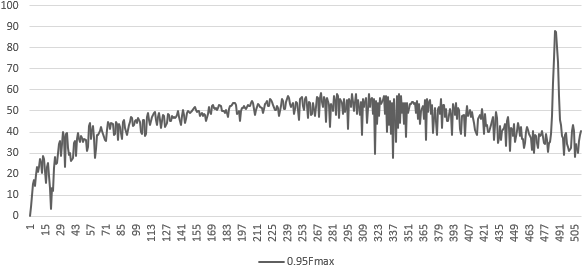
\includegraphics[width=0.99\linewidth]{../source/Udn.png}
	\caption{Power spectrum of U, time-warped downward test chirp}
	\label{fig:UdnSpec}
\end{figure}

\begin{figure}
	\centering
	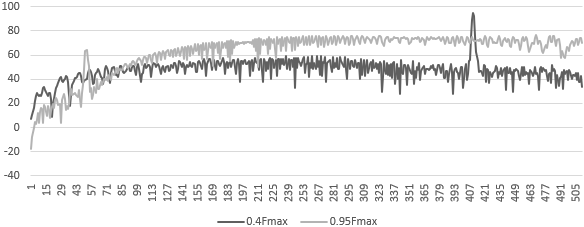
\includegraphics[width=0.99\linewidth]{../source/Uup.png}
	\caption{Power spectrum of U, time-warped upward test chirp}
	\label{fig:UupSpec}
\end{figure}

\subsubsection{Downsampling}

The i index is stepped from 0 to N-1, where N is a power of 2 (although it
doesn't have to be) for the convenience of the FFT. $\delta(i)$ sweeps
non-linearly from 0 to M. For each X, its index $\delta$ is the running sum
of $\lambda$. For each Y point, the downsampler averages one or more X points.

The most common downsampling method is a low pass filter whose output is
sampled less often than its input rate.
This method attenuates alias frequencies before they make it to the output.
Alias peaks don't correlate, but they do produce noise artifacts.
A biquad LPF is a good choice of filter because it uses coefficients that
can be stored in a table or computed in hardware.
The loss of endpoints due to the filter delay is not a problem.
The endpoints of the filtered X are allowed some slop,
as the Hann window will lop them off anyway.

Fractional interpolation sums $\lambda$ input samples of X.
This works without a filter so it's fast but noisy.
Some fractional arithmetic is required to handle partial contributions.
Fig.~\ref{fig:xint} illustrates a simple interpolation that adds two fractional
endpoints to 0 or more midpoints for downsampling.
$k$ is the integer part of $\delta$.

\begin{figure}
	\centering
	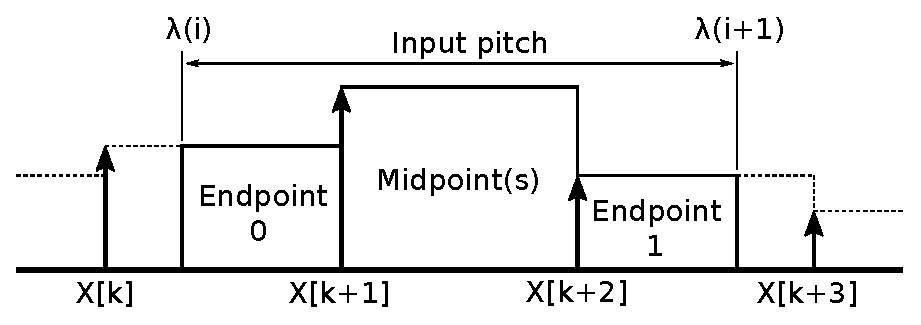
\includegraphics[width=0.95\linewidth]{../source/xint_e}
	\caption[X interpolation]{Sum of $X_\delta$ for downsampling}
	\label{fig:xint}
\end{figure}

In either case, the output of the downsampler could be scaled by
$s=\sqrt{1/\lambda}$ to flatten the noise floor.
The Central Limit Theorem reduces noise
by the square root of the number of samples in a sum.
On the other hand, one might expect energy conservation to cause the
amplitude of the incoming signal to fall off with time spreading.
So, the scaling should be optional.
Another instance of exponential sweep, with $\Lambda_s = -\Lambda/2$
and $s_0 = e^{R/2N}$,
can produce this scale factor rather easily.

\begin{figure}
	\centering
	\includegraphics[width=0.95\linewidth]{../source/xbuf_e}
	\caption[X buffer usage]{X buffer usage}
	\label{fig:xbuf}
\end{figure}

Oversampling would normally use a sliding window on a circular buffer sized as
a power of two to allow pointer wrapping by bitwise-and.
Fig.~\ref{fig:xbuf} shows the memory layout of $X$.
After a block of processing, $\alpha\Delta$ input samples are concatenated to
$X$ and the index of $X_0$ is offset by $\alpha\Delta$,
where $\Delta$ is the time interval of the blocks.

%%%%%%%%%%%%%%%%%%%%%%%%%%%%%%%%%%%%%%%%%%%%%%%%%%%%%%%%%%%%%%%%%%%%%%%%%%%%%%%
\subsection{FFT}

After X is time warped into Y, Y is processed by a Fast Fourier Transform and
converted to data set U containing N/2 frequency bins. Y and U may share the
same physical memory if the FFT is performed in place.
The output of the FFT is converted to the square of the magnitude,
so square root is not needed.

A pipelined FFT can be used so that the FFT isn't the bottleneck.
Throughput is then limited by downsampling, which when done in hardware
processes one $X$ sample per clock cycle.
This strategy offers the best performance in an ASIC implementation.

A Hann window $w(n)$ is applied to Y before performing the FFT.
\begin{equation}
w(n) = \frac{1}{2}\left(1 - cos\left( \frac{2\pi n}{N-1} \right)\right)
\end{equation}

A DIT FFT is the usual choice for RFFT since bit reversal is easier at the input.
With an RFFT, you get twice the outputs given real-only input.
Adjacent input samples are grouped as pairs, with even samples as real and odd
samples as imaginary components of the complex input points.
After a CFFT is performed, a separation step doubles the output size.
Our experience is that the precision of the separation step degrades with small N
(maybe we did it wrong), so a simple CFFT (with zeroed imaginary part)
may be preferable in cases of small N.

%%%%%%%%%%%%%%%%%%%%%%%%%%%%%%%%%%%%%%%%%%%%%%%%%%%%%%%%%%%%%%%%%%%%%%%%%%%%%%%%
\subsection{Upsampling}

U is upsampled to form time-domain signal V.
Let $\epsilon$ and j be the respective indices of U and V.
For every index $\epsilon$ of U, the corresponding frequency can be normalized
to a fraction $(\gamma)$ of $Fs/2$.

It's much easier to work in terms of exponents than logs,
so the preferred re-mapping (another exponential time-warping operation)
extracts $U[\epsilon]$ from a linear progression of $V[j]$.
Warp indexing uses the relation:
\begin{equation}
\epsilon = \left(\frac{N}{2}-1\right) e^{\omega(t - \tau)}
\end{equation}

Time t (scaled to match the output stream's sample rate) sweeps from $\tau$
in the opposite direction of R's sign,
causing the exponent to start at 1 and decay downward.

Up-sampling $U[\epsilon]$ to $V[j]$ can't use the popular interpolation scheme
(zero stuffing) because the interpolation factor must be irrational. Instead,
partial contributions to $V[j]$ are extracted from one or two U points by
interpolation.

$j$ sweeps downward from $\gamma(N/2-1)$.
Index $\epsilon(j)$ is independent of R.

\begin{equation}  \label{eq:eps_j}
\epsilon(j) = \gamma \left(\frac{N}{2}-1\right) e^{-kj/N}
\end{equation}

The desired difference between $\epsilon(0)$ and $\epsilon(1)$ in
Eq. \ref{eq:eps_j} is $1$. $\epsilon(0) = \gamma(N/2 - 1)$.

\begin{equation}
\epsilon(1) = \gamma(N/2 - 1) - 1 = \gamma(N/2 - 1) e^{-k/N}
\end{equation}

This gives a $k$ of approximately $2/\gamma$. The exact value is:

\begin{equation}
k = N \cdot ln \left( \frac{N-2}{N-2-(2/\gamma)} \right)
\end{equation}

As a sanity check of Eq. \ref{eq:eps_j}, $\epsilon(j)$ starts at (N/2-1) which
points to the highest frequency element of the FFT result.
It decays toward 0 but will never get there.
The number of elements in W memory is slightly less than N/2 to allow some I/O
headroom. Due to the limited size of W memory,
the lowest frequency is about $(1/e)$ of the highest frequency,
leaving the lower $\approx37$\% of the spectrum unused.

The exponential decay of $\epsilon$ can be handled by repeated multiplication,
one per $U[\epsilon]$ fetch.
The exponential sweep needs a small correction factor to have a base of exactly
$e$.
%\frac{N}{2} \cdot (1 - e^{-k})
Setting $e^{-k} = (1 + \zeta)^{N}$,
\begin{equation}
\zeta = e^{k/N} - 1
\end{equation}

Let $H_X$ be the integer number of new X samples per conversion.

Let $H_V$ be the real number of output samples per conversion.

\begin{equation}  \label{eq:hv}
H_V = H_X \cdot \frac{|R|}{k}
\end{equation}

\begin{figure}
	\centering
	\includegraphics[width=0.95\linewidth]{../source/uint_e}
	\caption[U interpolation]{Extraction of $U_\epsilon$}
	\label{fig:uint}
\end{figure}

Fig.~\ref{fig:uint} shows upsampling of U to V. It uses linear interpolation to
construct a curve to extract from.
In this case, the upsampler input pitch is less than 1.0 samples.
The height of $U_\epsilon$ is interpolated and multiplied by the pitch to get
the area under the curve, to be added to V[j].
The operation is similar to the "$\lambda < 1$" case of downsampling,
so the same hardware can support downsampling and upsampling.

Since $\epsilon$ is always positive, the upchirp case of $R>0$ needs to have its
j index mirrored by using V[v-j], where v is the maximum j such as (15/32)N.
The upsampler output is added to V memory as described below, indexed from the
top or bottom of the active region of V.

%%%%%%%%%%%%%%%%%%%%%%%%%%%%%%%%%%%%%%%%%%%%%%%%%%%%%%%%%%%%%%%%%%%%%%%%%%%%%%%%
\subsection{Correlation}

Warped U is added to output buffer V by RMS summation,
staggered in time (by $H_V$ samples) for each processing block.
When the downsampler's R value matches the chirp rate of an incoming chirp,
multiple peaks in the warped FFT output correlate in the output stream to
produce a corresponding output pulse in the V stream.
A more complex signal such as overlapping and/or modulated chirps will produce
pulse trains and/or modulation envelopes in the V stream.

\begin{figure}
	\centering
	\includegraphics[width=0.99\linewidth]{../source/wbuf_e}
	\caption[W correlation]{Correlation of V}
	\label{fig:wbuf}
\end{figure}

Fig.~\ref{fig:wbuf} shows the output correlator, another view of buffer V.
The output stream flows from left to right,
being initialized to 0 outside the accumulation region.
After $U_\epsilon$ is added to V, the $V_0$ index moves $H_V$ points
to the left, leaving $H_V$ newly minted output points.

Elements of V are accumulated squares of magnitudes.
An attempt was made to accumulate vectors,
with the idea that the phase rotations might sync up,
but it didn't work in simulation.
So, angle data from the FFT is discarded.

\section{QT Modulation}

Modulation is the reverse of demodulation.
It inputs a stream of (magnitude, angle) vectors and outputs a stream of real
samples. The downsample and upsample processes of modulation are the reverse
of demodulaton's upsample and downsample processes respectively.

\begin{figure}
	\centering
	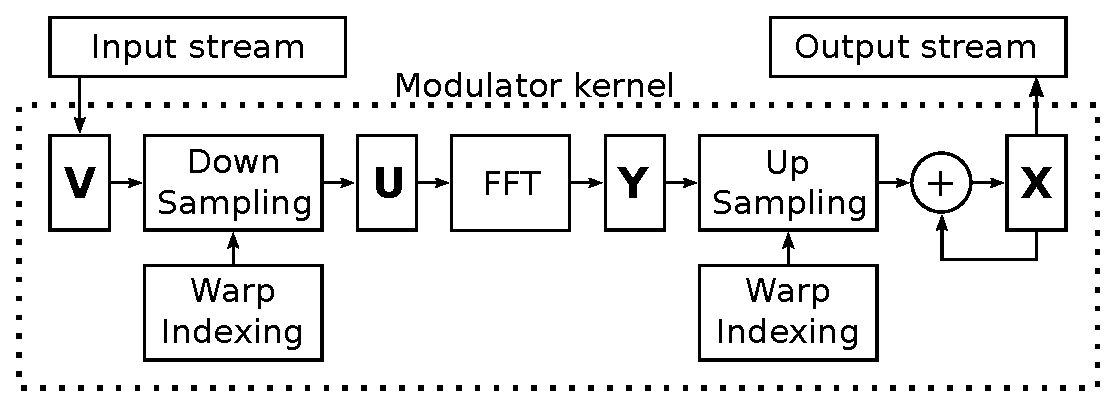
\includegraphics[width=0.95\linewidth]{../source/mod_e}
	\caption[Relative to Quantum Time Demodulation]{Modulation data flow}
	\label{fig:mod}
\end{figure}

%%%%%%%%%%%%%%%%%%%%%%%%%%%%%%%%%%%%%%%%%%%%%%%%%%%%%%%%%%%%%%%%%%%%%%%%%%%%%%%%
\subsection{Downsampling}

V is downsampled to form frequency-domain signal U.
Eq. \ref{eq:eps_j} relates integer index $j$ to fractional index $\epsilon(j)$.
Each point of V can be interpolated into a variable number of U points in a way
that accumulates V points and spits out U points as needed.

Another view is easier to describe mathematically, but needs a logarithm. Let
$\epsilon$ and j be the respective indices of U and V where $\epsilon/j < 1$.
$\epsilon$ is an integer that steps downward from $\epsilon_0$.
\begin{equation}
\epsilon_0 = \frac{N}{2} - 1
\end{equation}

Rewriting equation \ref{eq:eps_j} for $j(\epsilon)$,

\begin{equation}  \label{eq:j_eps}
j(\epsilon) = \left(\frac{N}{2}-1\right)
ln\left(\frac{\epsilon_0}{\epsilon}\right)
\end{equation}

The minimum $\epsilon$ is determined by the span of j.
Let j range from 0 to $v-1$ and $v = 0.469N$.

\begin{equation}
\epsilon(v-1) = \epsilon_0 e^\frac{-(v-1)}{0.5N - 1}
\end{equation}

\begin{equation}
\epsilon(0.469N) = \epsilon_0 e^\frac{-(0.469N-1)}{0.5N - 1}
\approx 0.391 \epsilon_0
\end{equation}

Since $\epsilon$ is always positive, the upchirp case of $R>0$ needs to have its
j index mirrored by using V[v-j], where v is the maximum j such as 0.469N.

%%%%%%%%%%%%%%%%%%%%%%%%%%%%%%%%%%%%%%%%%%%%%%%%%%%%%%%%%%%%%%%%%%%%%%%%%%%%%%%
\subsection{IFFT}

The IFFT ($U \rightarrow Y$) is an Inverse Fast Fourier Transform that
translates N/2 complex frequency values to N/2 complex points in the relative
time domain. These may be assumed to have Hermitian symmetry,
so the imaginary part of $Y$ can be ignored.
It's also possible to realize Y as N real points.

A Hann window is applied to Y after the FFT. Y is then warped and accumulated
in X in a manner similar to the demodulator's correlation function.

%%%%%%%%%%%%%%%%%%%%%%%%%%%%%%%%%%%%%%%%%%%%%%%%%%%%%%%%%%%%%%%%%%%%%%%%%%%%%%%%
\subsection{Upsampling}

The upsampling process of Fig.~\ref{fig:mod} translates the sample pitch of
Y to the sample pitch of X using the reverse of the downsampling process.

Fig.~\ref{fig:upsam} illustrates an interpolation scheme for recreating X from Y.
The slope calculation requires a $1/\lambda$ scale factor.
The expense of division can be avoided by using another instance of exponential
sweep such as that described by Eq. \ref{eq:lambdaApprox}.

The X points are the trapezoidal area under the curve in Fig.~\ref{fig:upsam}.
The \textit{Head} and \textit{Middle} regions produce output points.
The \textit{Tail} result is carried into the next \textit{Head}.

\begin{figure}
	\centering
	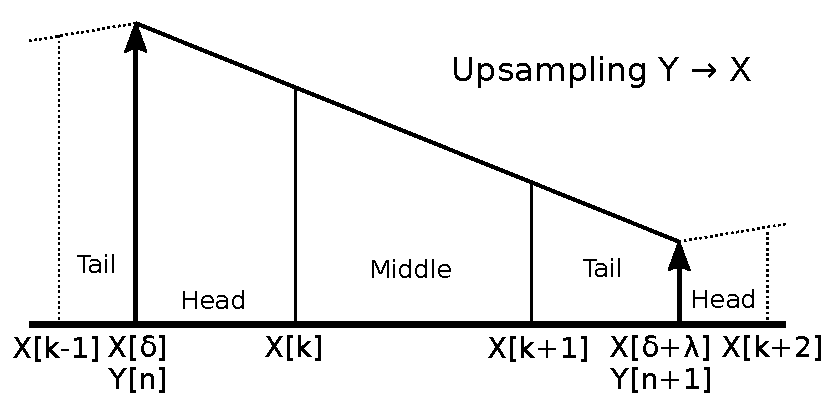
\includegraphics[width=0.8\linewidth]{../source/upsam_e}
	\caption[X interpolation]{Interpolation of Y for upsampling}
	\label{fig:upsam}
\end{figure}

Summation in X is similar to the data flow of Fig.~\ref{fig:wbuf},
but a little easier since X and Y are real (rather than complex) numbers.
X memory is wider than with demodulation to handle accumulation in memory.

\section{Testing}

The demodulation algorithm was tested by coding the algorithm in C99
(as a console application) and instrumenting it to display variables,
save arrays to files, benchmark the various stages, and generate bitmap images.

\subsection{Demodulation to Image}

The demodulation algorithm looks at the signal bandwidth between about
$\gamma F_S/5$ and $\gamma F_S/2$ where $\gamma$ is between 0.25 and 1.

Figure \ref{fig:chirpTest1} shows a spectrogram image of a noisy
negative-chirp test signal with R on the vertical axis.
$R=-0.2$ is at the top and $R=-0.78$ is at the bottom.
The output rates for each R are normalized (stretched at the low end)
to fit the image.
This gives the top of the image a fuzzy appearance.
A test signal was used to demonstrate detection of a chirp at
$R=-0.5$ and $N=4096$.
The chirp amplitude is 1/10 of the noise amplitude.
\begin{figure}
  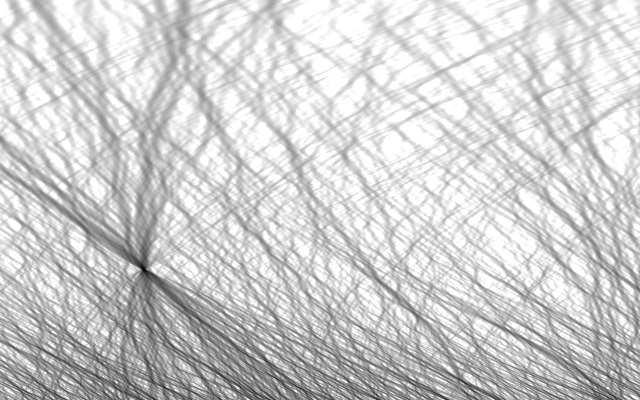
\includegraphics[width=\linewidth]{../source/chirp42m.jpg}
  \caption{Chirp power $(R<0)$ 20dB below noise.}
  \label{fig:chirpTest1}
\end{figure}

Noise has a cobweb-like look. A chirp shows up as a peak among the cobwebs.
To pick the chirp out of this mess, the peak is stored for each R value.
Figure \ref{fig:chirpRvalues1} shows the peak R values for a test chirp with a
power level 20, 25 and 30 dB below random noise.

\begin{figure}
  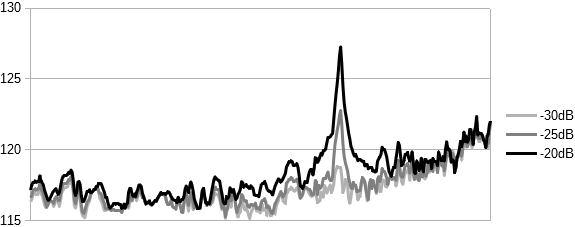
\includegraphics[width=\linewidth]{../source/Rpeaks.png}
  \caption{Peak power versus R}
  \label{fig:chirpRvalues1}
\end{figure}

\begin{figure}
  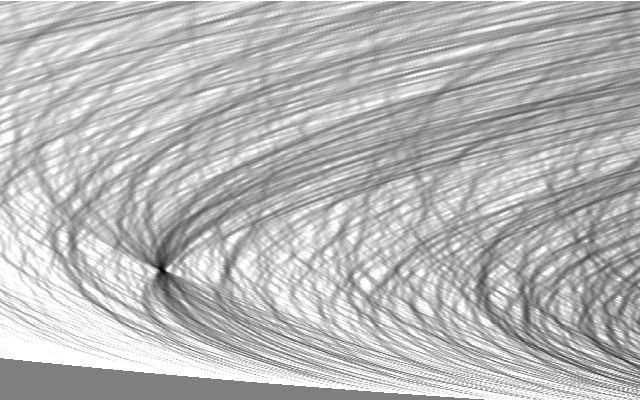
\includegraphics[width=\linewidth]{../source/chirp42p.jpg}
  \caption{Chirp power $(R>0)$ 25dB below noise.}
  \label{fig:chirpTest2}
\end{figure}

When the image uses positive chirp, the horizontal image follows $f_1$ rather 
than $f_0$. An R-dependent X offset is needed to make it reasonably viewable.
Figure \ref{fig:chirpTest2} shows a spectrogram image of a noisy positive-chirp
test signal.  



\bibliographystyle{IEEEtran}
\bibliography{IEEEabrv,../source/qtdsp}

\end{document}

